% !TEX root = ./main.tex
% !TEX encoding = UTF-8 Unicode
% !TEX program = pdflatex
% !TeX spellcheck = it_IT

\chapter{Caricamento dati}
In questo capitolo sono mostrate le operazioni effettuate per il caricamento
dei dati in MongoDB e per il suo collegamento a Databricks.

\section{Caricamento dati in MongoDB}
Come già detto in precedenza, MongoDB è stato installato su di un singolo nodo
e lanciato tramite il comando \textbf{\textit{mongod}}.\\
Su quest'istanza è stato possibile importare i dati in formato JSON.\\
Di seguito un esempio di import.

\begin{figure}[!htbp]
	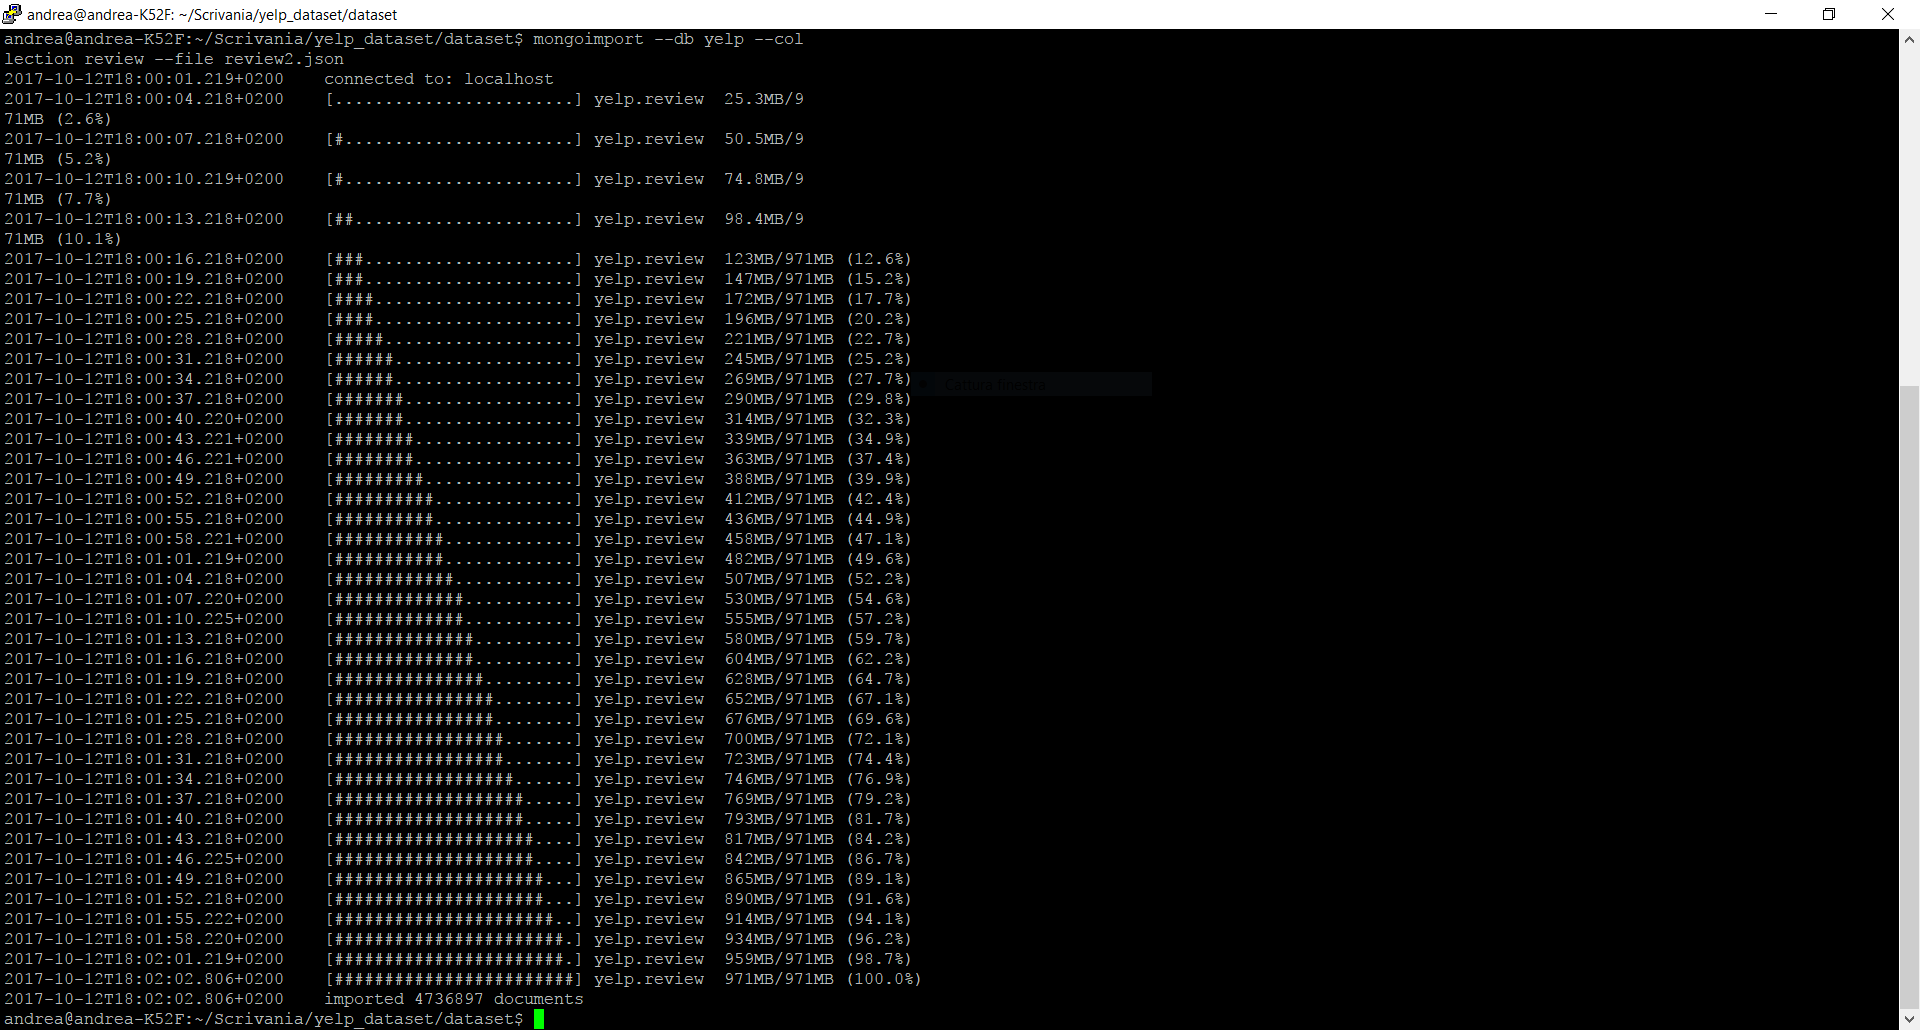
\includegraphics[width=.7\linewidth,keepaspectratio]{load_on_mongo}
  \caption{Apache Spark}
  \label{}
\end{figure}
\clearpage

\section{Da MongoDB a Databricks}

Per la connessione di MongoDB a Databricks è stato necessario scaricare il connettore.\\
Quest'ultimo fornisce le API necessarie per il collegamento e l'utlizzo dell'istanza del database.\\
In seguito è riportato il codice per la connessione a MongoDB e l'import dei dati.

\begin{figure}[!htbp]
  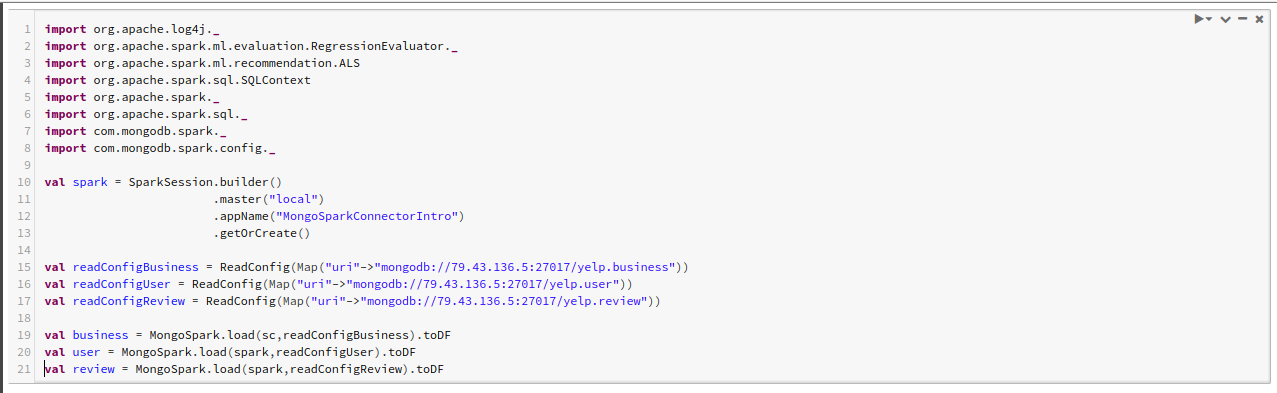
\includegraphics[width=1\linewidth,keepaspectratio]{mongo_spark}
  \caption{Codice per la connessione a MongoDB}
  \label{mongo_spark}
\end{figure}
